%--------------------------------------------------------------------
%                           Introduction
%--------------------------------------------------------------------
% This is an example of an unofficial University of Sydney LaTeX Beamer theme for the School of Mathematics and Statistics.

% Created by: Samantha Clarke
% Version: 0.1
% Updated: 9 May 2017
% Complied with: pdflatex

% GitHub repo: https://github.com/samanthalclarke/USYD-Beamer-Theme

% Please see the GitHub repo for current version, README.md, and licence.txt files. 

% This file can be redistributed and/or modified under the terms of the GNU Public License, version 3.

% Please note that this template is still under development. Any comments, feedback, additions, or suggestions are welcome. 

%--------------------------------------------------------------------
%                           Document Setup
%--------------------------------------------------------------------

\documentclass{beamer}
%\documentclass[handout]{beamer} 	%to produce printable hand-outs

% user packages
\usepackage[utf8]{inputenc}		% all displayable utf8 characters available as input
\usepackage[T1]{fontenc}		
\usepackage{hyperref}			% urls
\usepackage{amsmath,amssymb}
\usepackage{graphicx}			% graphics
\usepackage{color}
\usepackage{ulem}

% suppress navigation bar
\beamertemplatenavigationsymbolsempty

%% setting themes (inner & outer) - style definitions / changes
%\usetheme{usyd}							% use when doc setup is separated into .sty files
%\setbeamercolor{title}{fg=usydblack}		% note: not using title, author etc. ATM so not needed
%\setbeamercolor{author}{fg=usydblack}
\setbeamercolor{frametitle}{fg=usydred}
\setbeamercolor{alerted text}{fg=usydred}
%\useinnertheme{circles}
\setbeamercovered{transparent}				% use if you want greyed out steps rather than invisible

%\renewcommand\labelitemi{---}				% itemise as dashes - need to check if this works


% set fonts
\usefonttheme{structurebold}				% change font theme to Structurebold
\usefonttheme[onlymath]{serif}				% change math font theme to serif

% color definitions
\definecolor{usydred}{RGB}{230,70,38}
\definecolor{usydcharcoal}{RGB}{66,66,66}
\definecolor{usydblack}{RGB}{10,10,10}
\definecolor{usydwhite}{RGB}{255,255,255}
\definecolor{usydyellow}{RGB}{255,184,0}
\definecolor{usydblue}{RGB}{1,72,164}
\definecolor{usydgrey}{RGB}{241,241,241}

%--------------------------------------------------------------------
%                           Begin Document
%--------------------------------------------------------------------

\begin{document}

%--------------------------------------------------------------------
%                           Title Slide
%--------------------------------------------------------------------

% Set the background for the title slide.
\setbeamertemplate{background}
{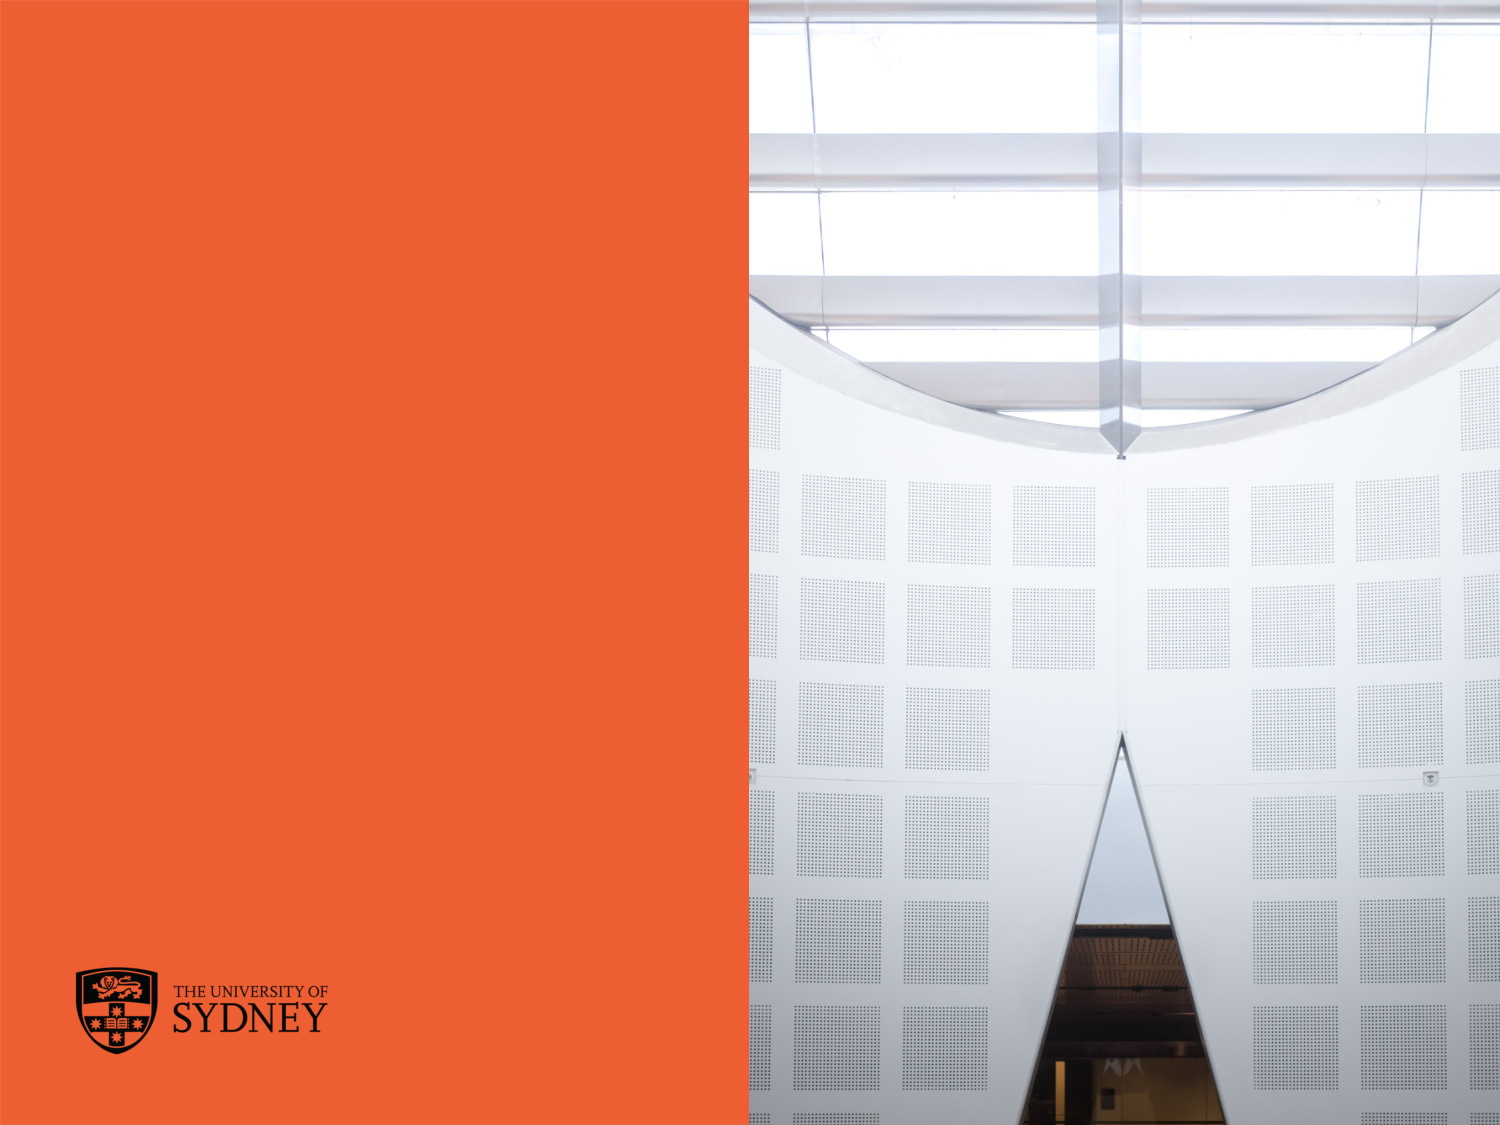
\includegraphics[width=\paperwidth,height=\paperheight]{titlebgstd2jun16.pdf}}
\setbeamertemplate{footline}[default]

\begin{frame}
\vspace{2cm}
\begin{columns}
\column{5.5cm}
{\bf{\color{usydwhite}Presentation Title}}	% Presentation Title
\vspace{1cm}
{\bf Presentation Subtitle}					% Presentation Subtitle
{\bf Presented by} \\
Professor Firstname Lastname \\				% Presenter Name
Faculty, Centre, or Unit					% Department

\column{6cm}
\end{columns}
\end{frame}

%--------------------------------------------------------------------
%                           Section Divider Slide
%--------------------------------------------------------------------

% Set the background for the section divider slide.
\setbeamertemplate{background}
{
\includegraphics[width=\paperwidth,height=\paperheight]{sectiondivstd2jun16.pdf}}
\setbeamertemplate{footline}[default]

\begin{frame}
\vspace{1cm}
\begin{columns}
\column{5.5cm}
{\bf{\color{usydwhite}Section Divider Heading}}	\\	% Section Divider Heading
{\color{usydwhite}Section Divider Subheading}		% Section Divider Subtitle

\column{6cm}
\end{columns}
\end{frame}


%-------------------------------------------------------------------
%                          Section 1
%-------------------------------------------------------------------
%
% Set the background for the rest of the slides.
\setbeamertemplate{background}[default]
\setbeamertemplate{footline}[default]
%\setbeamertemplate{footline}[frame number]		% need to rework this for footers: Page X 

\section{Section 1 Title}

%------------------------------ Slide ------------------------------%

\begin{frame}{Slide Heading A}

Here is a list:
\begin{itemize}
\item Item X.
\item Item Y.
\end{itemize}

\bigskip

A numbered list:
\begin{enumerate}
\item Point 1
\item Point 2
\end{enumerate}

\end{frame}

%------------------------------ Slide ------------------------------%

\begin{frame} 
\frametitle{Slide Heading B} 
\framesubtitle{The proof uses \textit{reductio ad absurdum}.} 

\begin{theorem}
There is no largest prime number. \end{theorem} 
\begin{enumerate} 
\item<1-| alert@1> Suppose $p$ were the largest prime number. 
\item<2-> Let $q$ be the product of the first $p$ numbers. 
\item<3-> Then $q+1$ is not divisible by any of them. 
\item<1-> But $q + 1$ is greater than $1$, thus divisible by some prime
number not in the first $p$ numbers.
\end{enumerate}

\end{frame}

%------------------------------- End -------------------------------%

\end{document}

